\section{Statistical Analysis}
\label{sec:analysis}

In this section, we delve into a comprehensive analysis of the retrieval effectiveness for our 5 different runs submitted to \ac{CLEF} on both the French and English collections (see Table \ref{tab:run_parameters}). 
The analysis aims to evaluate the performance of different runs and provides insights into the effectiveness of the system in retrieving and ranking relevant documents.

We begin by analyzing the results obtained from the French collection. 
The overall \ac{nDCG} and \ac{MAP} comparison allows us to gain an initial understanding of the performance differences between runs 2, 3, and 5, considering short-term, heldout, and long-term evaluations. 
By examining the \ac{nDCG} scores and \ac{RnD} values, we can identify the run that demonstrates the highest effectiveness in retrieving relevant documents.

Furthermore, we employ two-way \ac{ANOVA} tests to investigate the significance of the observed differences in the long-term and short-term evaluations.
Along with this, the analysis also includes the implementation of the \acl{THSD} test, a post-hoc analysis for \ac{ANOVA} that compares group means while controlling for multiple comparisons, ensuring reliable identification of significant differences.

This analysis provides valuable insights into the performance of the \ac{IR} system on the French collection, guiding us in identifying areas for improvement.

Subsequently, we shift our focus to the analysis of results obtained from the English collection. 
We conduct an analogous evaluation, comparing the performance of runs 1 and 4 in the same way as stated above for the French collection. 

Still, we put here an extract of the first three columns of Table \ref{tab:results_submission_heldout}, which can be seen as a sort of recap to have at hand of our runs submitted to \ac{CLEF}:

\begin{table}[!h]
    \centering
    \begin{tabular}{ |c|c|c| }
        \hline
        \hline
        \multicolumn{3}{|c|}{heldout} \\ \hline
        run  & language & type \\ \hline
        run2 &   FR   & QUEREXPANSION \\
        run3 &   FR   & RERANKING \\
        run5 &   FR   & SBERT\_BM25 \\
        \hline
        run1 &   EN   & JSCLEANER\_BM25 \\
        run4 &   EN   & RERANKING\_ENGLISH \\
        \hline
    \end{tabular}
    \caption{Recap of our runs submitted to \ac{CLEF}.}
    \label{tab:runs_recap}
\end{table}

\newpage
\subsection{Analysis of Results on the French Collection}
\enlargethispage{5\baselineskip}
\subsubsection{Overall \textit{nDCG} Comparison}  \label{sec:ndcg_comparison_french}

The overall \ac{nDCG} comparison of runs 2, 3, and 5 on the French collection is presented in Figure \ref{fig:overall_ndcg_french_boxplot}. 
This boxplot provides valuable insights into the performance of each run, with the bars representing the \ac{nDCG} scores for each run. 
The color coding distinguishes the different evaluation periods, with short-term depicted in green, heldout in orange, and long-term in pink. 
The delta values within the boxes represent the \ac{RnD} of each run compared to the heldout run.

\begin{figure}[!h]
\centering
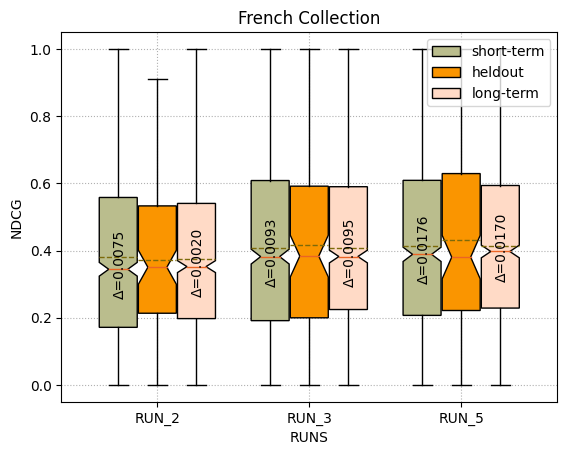
\includegraphics[width=0.8\textwidth]{figure/StatisticalAnalysis/BoxPlot/NDGC French.png}
\caption{Overall \ac{nDCG} Comparison for runs 2, 3, and 5 on the French Collection}
\label{fig:overall_ndcg_french_boxplot}
\end{figure}

Analyzing the overall \ac{nDCG} comparison, we observe that runs 3 and 5 consistently outperform run 2 across both short and long-term evaluations. 
These runs achieve higher \ac{nDCG} scores, indicating their superior effectiveness in capturing and ranking relevant documents. 
The fact that both runs 3 and 5 exhibit similar levels of performance suggests comparable retrieval capabilities among these two.

However, when considering the \ac{RnD} values, we observe some variations among the runs. 
Run 5 demonstrates a noticeable drop in \ac{nDCG} compared to the heldout run, as indicated by the \ac{RnD} delta values. 
This indicates a potential decrease in retrieval performance when transitioning from the heldout period to the short and long term.

On the other hand, run 3 displays a relatively smaller drop in \ac{nDCG} compared to the heldout run, suggesting greater stability and consistency in performance.

In contrast, run 2 exhibits relatively lower \ac{nDCG} scores, particularly in the long-term evaluation. This can be attributed to its more greedy approach, which might compromise its ability to retrieve relevant documents as the collection evolves over time.


\newpage
\enlargethispage{7\baselineskip}
\subsubsection{Overall \textit{MAP} Comparison} \label{sec:map_comparison_french}
The boxplot shown in Figure \ref{fig:map_french} presents the overall \ac{MAP} comparison of runs 2, 3, and 5 on the French Collection.
The notation for the used colors is the same as for Figure \ref{fig:overall_ndcg_french_boxplot}.
From the boxplot, we can observe the distribution of \ac{MAP} scores for each run and collection type. The height of each box indicates the \ac{IQR}, representing the range of the middle 50\% of the data. 
The horizontal line within each box corresponds to the median value, while the whiskers above and below the box extend to the highest and lowest values within 1.5 times the \ac{IQR}.

\begin{figure}[!h]
    \centering
    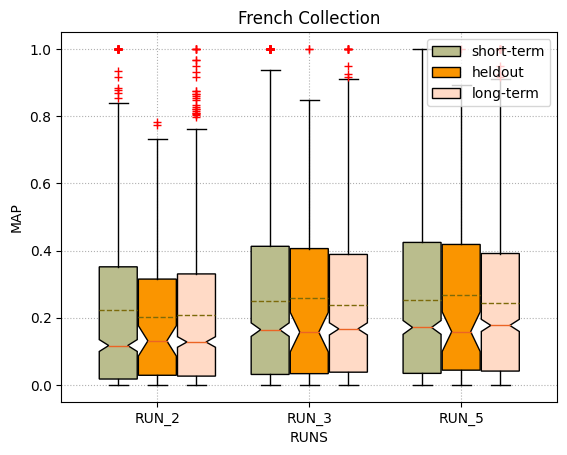
\includegraphics[width=0.8\textwidth]{figure/StatisticalAnalysis/BoxPlot/MAP French.png}
    \caption{Overall MAP Comparison of runs 2, 3, and 5 on the French Collection}
    \label{fig:map_french}
\end{figure}

Analyzing the overall \ac{MAP} comparison, we observe that runs 3 and 5 consistently outperform run 2 across both short and long-term evaluations, similarly to what we have seen in Section \ref{sec:ndcg_comparison_french}.
These runs achieve higher \ac{MAP} scores, indicating their superior effectiveness in accuracy.  

However, we can see that run 5 demonstrates a noticeable drop in \ac{MAP} of the long-term compared to the heldout run. 
This indicates a potential decrease in retrieval performance when transitioning from the heldout period to the long term. 
On the other hand, run 3 displays a relatively smaller drop in \ac{MAP} compared to the heldout run, suggesting greater stability and consistency in capturing relevant documents over time.

These results, together with the ones we have seen on \ac{nDCG} in Section \ref{sec:ndcg_comparison_french}, suggests that the changes done from run 3 to run 5 for sure led to improvements, but they have to be better optimized towards temporal persistence.

In contrast, run 2 exhibits relatively lower \ac{MAP} scores, particularly in the long-term evaluation. The reasons to which this can be attributed are the same stated in Section \ref{sec:ndcg_comparison_french}.

Overall, these results confirm what we found in Section \ref{sec:ndcg_comparison_french}: runs 3 and 5 are competitive with each other, while run 2 exhibits lower performances compared to these, due to its more basic implementation (see Table \ref{tab:run_parameters}). 


\subsubsection{Two-way \textit{ANOVA} on the Long Term French Collection} \label{sec:anova_fr_lt}

The results of the two-way \ac{ANOVA} conducted on the Long Term French Collection are depicted in Figure \ref{fig:lt_anova_french}, which showcases the \ac{nDCG} and \ac{AP} scores for run 2 in red, run 3 in grey, and run 5 in blue. 
These plots enable us to examine the effects of both the run choice and the long-term evaluation on the performances.

\begin{figure}[!h]
    \centering
    \begin{subfigure}[b]{0.49\textwidth}
      \centering
      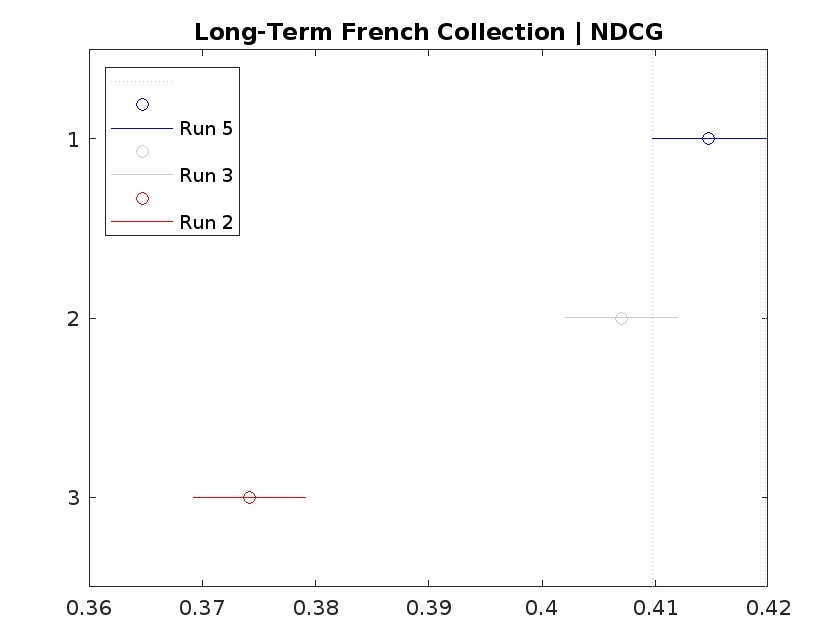
\includegraphics[width=\textwidth]{figure/StatisticalAnalysis/ANOVA 2/ndcg-lt-fr.jpeg}
      %\caption{\ac{nDCG} Two-way \ac{ANOVA} for Runs 2, 3, and 5 on the Long Term French Collection}
      \label{fig:lt_anova_french_ndcg}
    \end{subfigure}
    \hfill
    \begin{subfigure}[b]{0.49\textwidth}
      \centering
      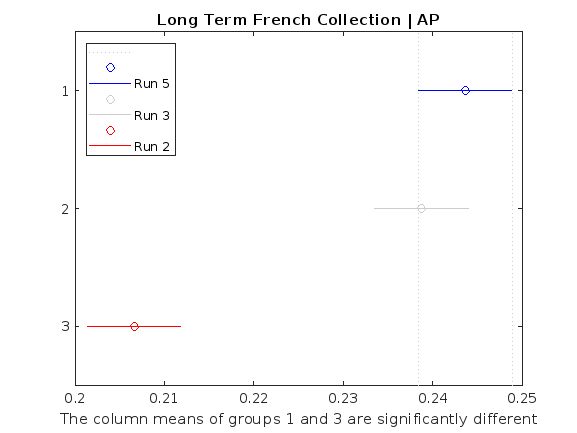
\includegraphics[width=\textwidth]{figure/StatisticalAnalysis/ANOVA 2/ap-lt-fr.jpeg}
      %\caption{\ac{AP} Two-way \ac{ANOVA} for Runs 2, 3, and 5 on the Long Term French Collection}
      \label{fig:lt_anova_french_ap}
    \end{subfigure}
    \caption{Two-way \ac{ANOVA} plots for the runs on the French Collection}
    \label{fig:lt_anova_french}
  \end{figure}

Analyzing the two-way \ac{ANOVA} plot above, at first view we can notice, as expected, that there is no interaction among the three runs.  

Then, we observe that run 5 consistently achieves the highest \ac{nDCG}  and \ac{AP} scores across different evaluation points. 
Run 2 exhibits lower performance compared to the other runs, while run 3 shows a relatively stable performance, albeit slightly lower than Run 5, confirming what we found in Sections \ref{sec:ndcg_comparison_french} and \ref{sec:map_comparison_french}.
In addition, the overlap we find among the columns of run 3 and run 5 suggests that the small changes done among these two (see Table \ref{tab:run_parameters}) led to some small albeit noticeable improvements. 
These findings suggest that both the choice of run and the long-term evaluation have a significant impact on the overall \ac{nDCG} and \ac{AP} scores obtained.

To complement the two-way \ac{ANOVA} plots, we refer to Tables \ref{table:lt_anova_french} and \ref{table:lt_anova_french_ap}, that provide multiple comparisons between the \ac{nDCG} and \ac{AP} scores, variance, and p-values associated with runs 2, 3, and 5. 

The tables present the results of the pairwise comparisons between different runs. 
The "\textit{Run A}" and "\textit{Run B}" columns indicate the runs being compared.
The "\textit{Lower Limit}" and "\textit{Upper Limit}" columns represent the lower and upper bounds of the confidence interval, while the "\textit{A-B}" column indicates the mean difference between the runs.
The "\textit{P-value}" column displays the statistical significance of the comparison, indicating the level of significance and suggesting whether there is a significant difference in performance between runs.

\newpage
\begin{table}[!h]
    \centering
    \caption{\ac{nDCG} Multiple Comparisons for runs 2, 3, and 5 on the Long Term French Collection}
    \label{table:lt_anova_french}
    \begin{tabular}{cccccc}
    \hline
    Run A & Run B & Lower Limit & A-B & Upper Limit & P-value \\ \hline
    5 & 3 & -0.0023 & 0.0077 & 0.0177 & 0.1661 \\
    5 & 2 & 0.0305 & 0.0405 & 0.0505 & $1.16 \cdot 10^{-21}$ \\
    3 & 2 & 0.0228 & 0.0328 & 0.0428 & $3.84 \cdot 10^{-14}$ \\ \hline
    \end{tabular}
\end{table}

\begin{table}[!h]
    \centering
    \caption{\ac{AP} Multiple Comparisons for runs 2, 3, and 5 on the Long Term French Collection}
    \label{table:lt_anova_french_ap}
    \begin{tabular}{cccccc}
    \hline
    Run A & Run B & Lower Limit & A-B & Upper Limit & P-value \\ \hline
    5 & 3 & -0.0057 & 0.0049 & 0.0154 & 0.523 \\
    5 & 2 & 0.0265 & 0.037 & 0.0476 & $3.57 \cdot 10^{-16}$ \\
    3 & 2 & 0.0216 & 0.0322 & 0.0427 & $2.50 \cdot 10^{-12}$ \\ \hline
    \end{tabular}
\end{table}

Looking at Table \ref{table:lt_anova_french}, the comparison between run 5 and run 3 yields a \textit{p-value} of 0.1661, indicating that the mean difference in \ac{nDCG} scores between these runs is not statistically significant.
Similarly, the comparison between run 5 and run 2 results in an extremely low \textit{p-value} of $1.16 \cdot 10^{-21}$, suggesting a highly significant difference in \ac{nDCG} scores.
Finally, the comparison between run 3 and run 2 also demonstrates a remarkably low \textit{p-value} of $3.84 \cdot 10^{-14}$, indicating a significant discrepancy in their \ac{nDCG} scores.

The results displayed in Table \ref{table:lt_anova_french_ap} don't say anything new except to confirm what is stated above.

Finally, the p-values obtained from the comparisons reinforce the observations made from the two-way \ac{ANOVA} plot, highlighting the superior performance of Run 5 and the relatively stable performance of Run 3 compared to the other runs.

\newpage
\enlargethispage{10\baselineskip}
\subsubsection{Two-way ANOVA on the Short Term French Collection}

Similarly, the results of the two-way \ac{ANOVA} for \ac{nDCG} and \ac{AP} performed on the Short Term French Collection are visualized in Figure \ref{fig:st_anova_french}.

\begin{figure}[!h]
    \centering
    \begin{subfigure}[b]{0.49\textwidth}
        \centering
        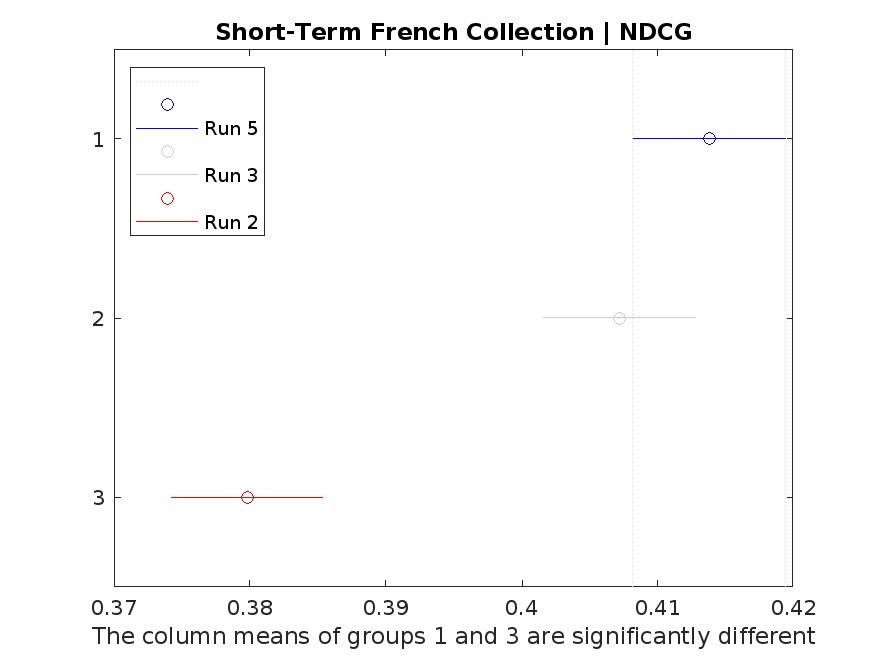
\includegraphics[width=\textwidth]{figure/StatisticalAnalysis/ANOVA 2/ndcg-st-fr.jpeg}
        %\caption{Two-way \ac{ANOVA} for Runs 2, 3, and 5 on the Short Term French Collection}
        \label{fig:st_anova_french_ndcg}
    \end{subfigure}
    \hfill
    \begin{subfigure}[b]{0.49\textwidth}
        \centering
        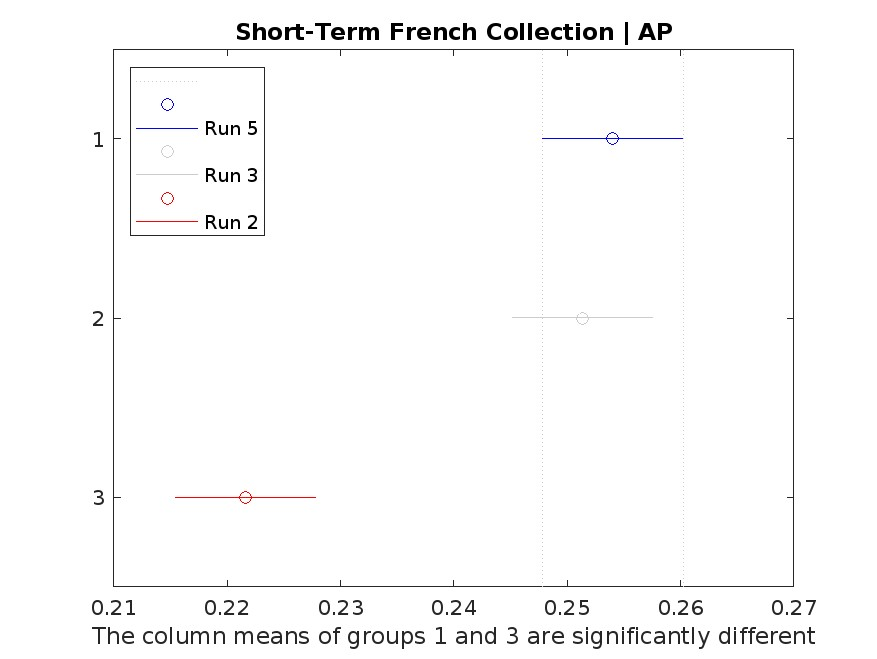
\includegraphics[width=\textwidth]{figure/StatisticalAnalysis/ANOVA 2/ap-st-fr.jpeg}
        %\caption{Two-way \ac{ANOVA} for Runs 2, 3, and 5 on the Short Term French Collection}
        \label{fig:st_anova_french_ap}
    \end{subfigure}
    \caption{Two-way \ac{ANOVA} for runs 2, 3, and 5 on the Short Term French Collection}
    \label{fig:st_anova_french}
\end{figure}

Looking at Figure \ref{fig:lt_anova_french}, we can see that the results above obtained on the short-term Collection are almost identical.
Therefore, the considerations made in Section \ref{sec:anova_fr_lt} hold in almost the same way for the results the system got on short-term Collection.

To further investigate the statistical differences among the runs, we refer to the multiple comparisons Tables \ref{table:st_anova_french} and \ref{table:st_anova_french_ap} shown below, which uses the same notation as Table \ref{table:lt_anova_french}:

\begin{table}[!h]
    \centering
    \caption{\ac{nDCG} Multiple Comparisons for runs 2, 3, and 5 on the Short Term French Collection}
    \label{table:st_anova_french}
    \begin{tabular}{cccccc}
    \hline
    Run A & Run B & Lower Limit & A-B & Upper Limit & P-value \\ \hline
    5 & 3 & -0.0042 & 0.0067 & 0.0177 & 0.3215 \\
    5 & 2 & 0.0232 & 0.0341 & 0.0451 & $7,97 \cdot 10^{-13}$ \\
    3 & 2 & 0.0164 & 0.0274 & 0.0384 & $1.39 \cdot 10^{-8}$ \\ \hline
    \end{tabular}
\end{table}

\begin{table}[!h]
    \centering
    \caption{\ac{AP} Multiple Comparisons for runs 2, 3, and 5 on the Long Term French Collection}
    \label{table:st_anova_french_ap}
    \begin{tabular}{cccccc}
    \hline
    Run A & Run B & Lower Limit & A-B & Upper Limit & P-value \\ \hline
    5 & 3 & -0.0095 & 0.0027 & 0.0148 & 0.8631 \\
    5 & 2 & 0.0203 & 0.0324 & 0.0445 & $1.18 \times 10^{-9}$ \\
    3 & 2 & 0.0176 & 0.0297 & 0.0419 & $2.87 \times 10^{-8}$ \\ \hline
    \end{tabular}
\end{table}

Looking at Table \ref{table:st_anova_french}, the comparison between run 5 and run 3 yields a \textit{p-value} of 0.355, indicating that the mean difference in \ac{nDCG} scores between these runs is not statistically significant.
Similarly, the comparison between run 5 and run 2 results in a remarkably low \textit{p-value} of $3.86 \cdot 10^{-12}$, suggesting a highly significant difference in \ac{nDCG} scores.
Finally, the comparison between run 3 and run 2 also demonstrates a low \textit{p-value} of $3.33 \cdot 10^{-8}$, indicating a significant discrepancy in their \ac{nDCG} scores.

In summary, the statistical analysis of the results obtained on the French collection revealed that run 5 is the most effective one among the three, showing a noticeable overall strength in retrieving and ranking relevant documents.
This was easily predictable since this is the last and most elaborate and promising implementation we did for the French Collection, as discussed in Section \ref{sec:results}.
Anyway, by boxplots in Sections \ref{sec:ndcg_comparison_french} and \ref{sec:map_comparison_french} emerged that our \ac{IR} system can still be optimized towards persistence over time.


\newpage
\enlargethispage{8\baselineskip}
\subsection{Analysis of Results on the English Collection}

\subsubsection{Overall \textit{nDCG} Comparison} \label{sec:ndcg_comparison_eng}

The overall \ac{nDCG} comparison for runs 1 and 4 on the English collection is depicted in Figure \ref{fig:overall_ndcg_eng}, which uses the same notation as Figure \ref{fig:overall_ndcg_french_boxplot}.

\begin{figure}[!h]
\centering
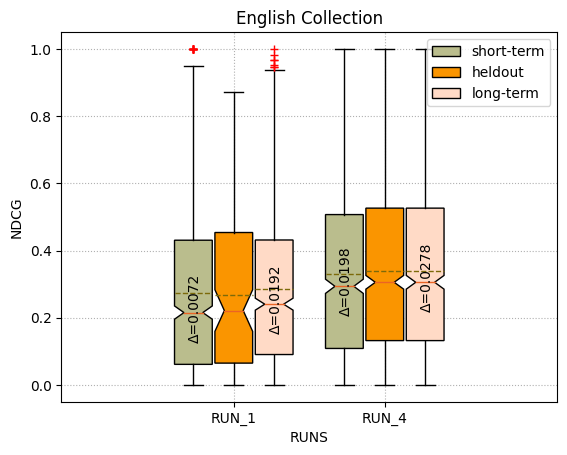
\includegraphics[width=0.8\textwidth]{figure/StatisticalAnalysis/BoxPlot/NDGC ENGLISH.png}
\caption{Overall nDCG Comparison for runs 1 and 4 on the English Collection}
\label{fig:overall_ndcg_eng}
\end{figure}

Upon analyzing the overall \ac{nDCG} comparison, we first notice that the results on the English Collection are notably worse compared to those observed for the French Collection in Section \ref{sec:ndcg_comparison_french}.
This discrepancy is not unexpected, since we focused most of our work into improving the retrieval and ranking performances of our \ac{IR} system on the French Collection.

Examining the boxplot in Figure \ref{fig:overall_ndcg_eng}, we can observe that run 4 consistently outperforms run 1 and achieves higher \ac{nDCG} scores across both the Short and Long Term evaluations on the English Collection.
The clear separation between the two runs in the boxplot suggests significant differences in their retrieval performance, indicating the superior effectiveness of Run 4 in retrieving relevant documents.

Furthermore, by considering the \ac{RnD} deltas represented by the values inside the boxes, we can observe that run 4 exhibits a good level of stability between the Short and Long Term evaluations, with minimal changes in its \ac{nDCG} scores.
On the other hand, run 1 shows a notable increase in \ac{RnD} from the Short to the Long Term, more than doubling the delta value.
This indicates that run 1's performance significantly deteriorates when transitioning from the Short to the Long Term evaluation of the English Collection.

In summary, the overall \ac{nDCG} comparison confirms that run 4 performs better than run 1 in all evaluation settings on the English Collection.
Run 4 demonstrates higher \ac{nDCG} scores and exhibits greater stability between the Short and Long Term evaluations, while run 1 experiences a noticeable decline in performance when moving from the Short to the Long Term.
These findings highlight the importance of the improvements achieved in run 4 and emphasize its superior retrieval effectiveness compared to run 1.

\newpage
\enlargethispage{6\baselineskip}
\subsubsection{Overall \textit{MAP} Comparison} \label{sec:map_comparison_eng}

We now turn our attention to the overall \ac{MAP} comparison of runs 1 and 4 on the English collection, as illustrated in Figure \ref{fig:map_english}.
The boxplot showcases the distribution of \ac{MAP} scores, using the same notation as Figure \ref{fig:map_french}.

\begin{figure}[!h]
\centering
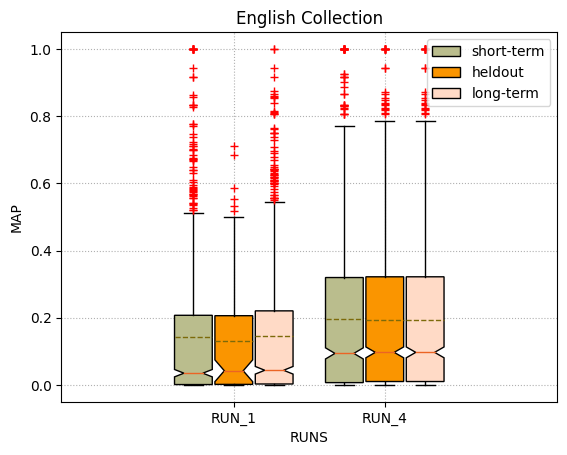
\includegraphics[width=0.8\textwidth]{figure/StatisticalAnalysis/BoxPlot/MAP English.png}
\caption{Overall \ac{MAP} Comparison of runs 1 and 4 on the English Collection}
\label{fig:map_english}
\end{figure}

Analyzing the boxplot in Figure \ref{fig:map_english}, we observe that run 4 consistently outperforms run 1 on all three collections: Short Term, Heldout, and Long Term.
Run 4 exhibits higher median \ac{MAP} scores in both the Short Term and Long Term evaluations, indicating its better overall effectiveness in retrieving relevant documents on the English Collection.

However, in terms of the Heldout Collection, both runs 1 and 4 display comparable median \ac{MAP} scores, indicating similar retrieval performance within this collection.

It's also noticeable how run 1 slightly reaches a \ac{MAP} score of 20\%, while run 4 is able to reach around 30\% on all the time periods considered.

These findings reinforce the conclusions drawn in Section \ref{sec:ndcg_comparison_eng} regarding the superior performance of run 4 compared to run 1 on the English Collection.


\newpage
\enlargethispage{8\baselineskip}
\subsubsection{Two-way \textit{ANOVA} on the Long Term English Collection}

The results of the two-way \ac{ANOVA} performed on the Long Term English Collection are shown in Figure \ref{fig:lt_anova_eng}, which illustrates the \ac{nDCG} and \ac{AP} scores for Run 1 in red on the left and Run 4 in blue on the right.

\begin{figure}[!h]
    \centering
    \begin{subfigure}[b]{0.49\textwidth}
        \centering
        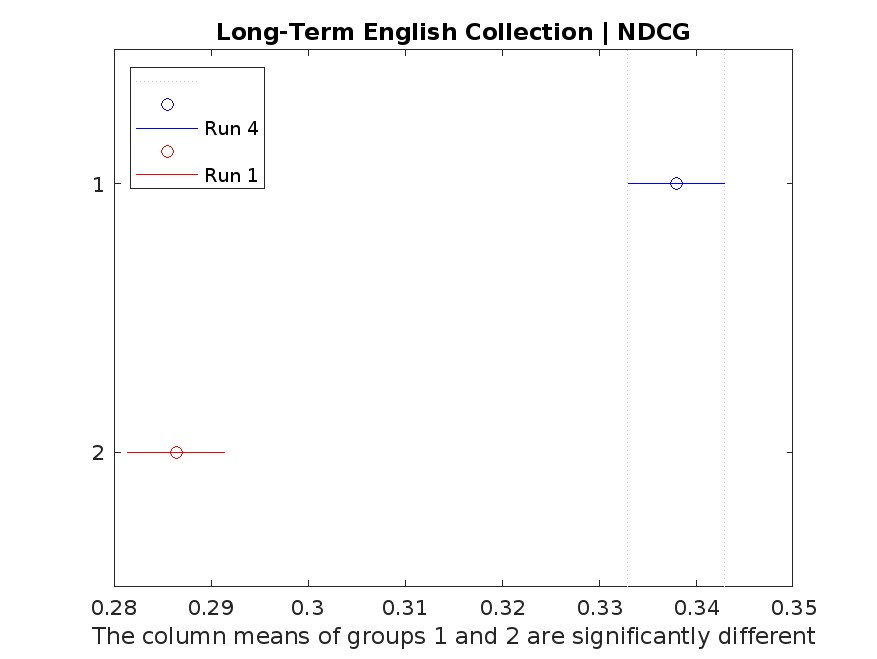
\includegraphics[width=\textwidth]{figure/StatisticalAnalysis/ANOVA 2/ndcg-lt-en.jpeg}
        %\caption{Two-way ANOVA for Runs 1 and 4 on the Long Term English Collection}
        \label{fig:lt_anova_eng_ndcg}
    \end{subfigure}
    \hfill
    \begin{subfigure}[b]{0.49\textwidth}
        \centering
        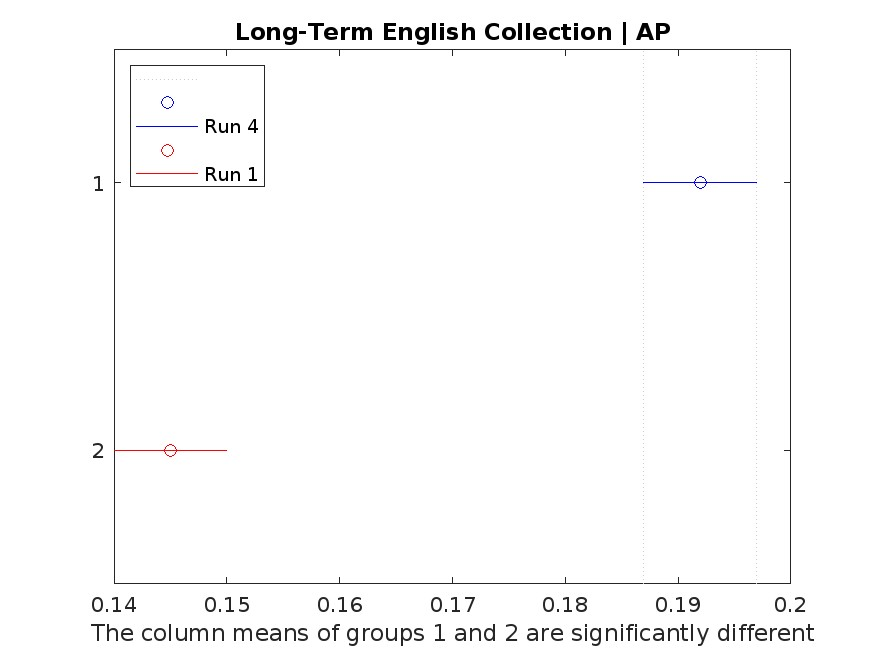
\includegraphics[width=\textwidth]{figure/StatisticalAnalysis/ANOVA 2/ap-lt-en.jpeg}
        %\caption{Two-way ANOVA for Runs 1 and 4 on the Long Term English Collection}
        \label{fig:lt_anova_eng_ap}
    \end{subfigure}
    \caption{Two-way ANOVA for runs 1 and 4 on the Long Term English Collection}
    \label{fig:lt_anova_eng}
\end{figure}

At first, we can see that, as expected, there is no interaction between these two runs. To reinforce this, we can also see that there is no overlap between their column means.
This was fairly expectable, since the improvements done from run 1 to run 4 are numerous (see Table \ref{tab:run_parameters}).

Continuing into analyzing the two-way \ac{ANOVA} plot, we find that run 4 achieves higher \ac{nDCG} scores compared to run 1 across different evaluation points.
This suggests the superiority of run 4 in retrieving relevant documents in the long term on the English collection, keep confirming what we found in Section \ref{sec:ndcg_comparison_eng}.

To provide additional statistical information, we refer to Tables \ref{table:lt_anova_eng} and \ref{table:lt_anova_eng_ap}, which present the results of multiple comparisons between run 1 and run 4 for the Long Term English Collection.
The tables show the lower limit, A-B difference, upper limit, and p-value for the comparisons.
In this case, the table presents a single row since it consists in only one comparison between two runs.

\begin{table}[!h]
    \centering
    \caption{\ac{nDCG} Multiple comparisons for the Long Term English Collection}
    \label{table:lt_anova_eng}
    \begin{tabular}{cccccc}
    \hline
    Run A & Run B & Lower Limit & A-B Difference & Upper Limit & P-value \\
    \hline
    4 & 1 & 0.0409 & 0.0508 & 0.0608 & $1.49 \times 10^{-24}$ \\
    \hline
    \end{tabular}
\end{table}

\begin{table}[!h]
    \centering
    \caption{\ac{AP} Multiple comparisons for the Long Term English Collection}
    \label{table:lt_anova_eng_ap}
    \begin{tabular}{cccccc}
    \hline
    Run A & Run B & Lower Limit & A-B Difference & Upper Limit & P-value \\
    \hline
    4 & 1 & 0.0364 & 0.0464 & 0.0565 & $4.44 \times 10^{-20}$ \\
    \hline
    \end{tabular}
\end{table}

Table \ref{table:lt_anova_eng} suggests a significant difference between run 1 and run 4 in terms of \ac{nDCG} scores for the Long Term English Collection.
The positive A-B difference indicates that run 4 consistently achieves higher \ac{nDCG} scores than run 1 across different evaluation points. This consideration is further supported by the small p-value of $6.77 \times 10^{-25}$.

These findings further support the conclusion that run 4 performs better than run 1 in terms of retrieving relevant documents over the long term on the English collection, as discussed in Sections \ref{sec:ndcg_comparison_eng} and \ref{sec:map_comparison_eng}.


\newpage
\enlargethispage{5\baselineskip}
\subsubsection{Two-way \textit{ANOVA} on the Short Term English Collection}

Similarly, the results of the two-way \ac{ANOVA} for \ac{nDCG} and \ac{AP} performed on the Short Term English Collection are depicted in Figure \ref{fig:st_anova_eng}.

\begin{figure}[!h]
    \centering
    \begin{subfigure}[b]{0.49\textwidth}
        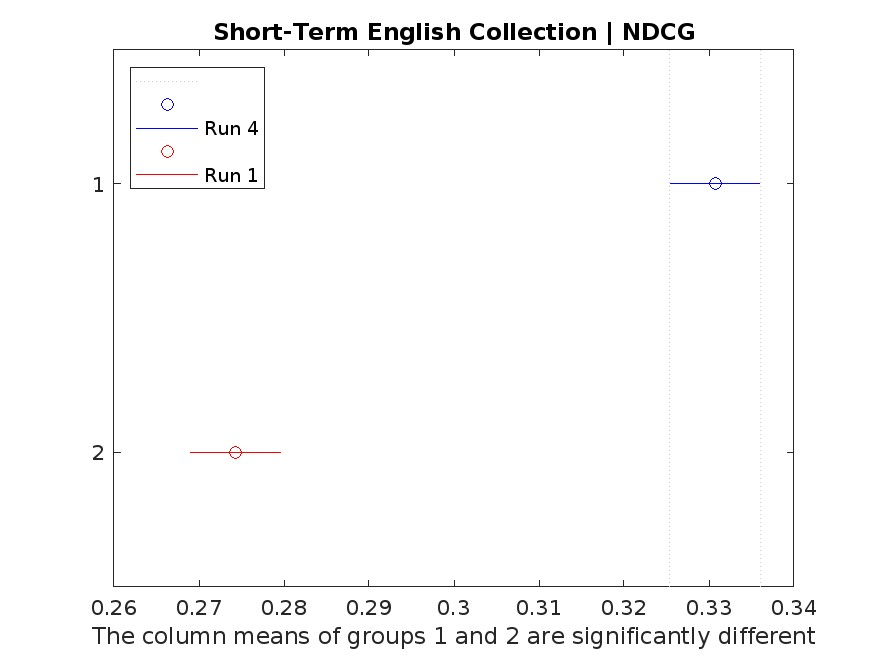
\includegraphics[width=\textwidth]{figure/StatisticalAnalysis/ANOVA 2/ndcg-st-en.jpeg}
        %\caption{Two-way ANOVA for Runs 2 and 4 on the Short Term English Collection}
        \label{fig:st_anova_eng_ndcg}
    \end{subfigure}
    \hfill
    \begin{subfigure}[b]{0.49\textwidth}
        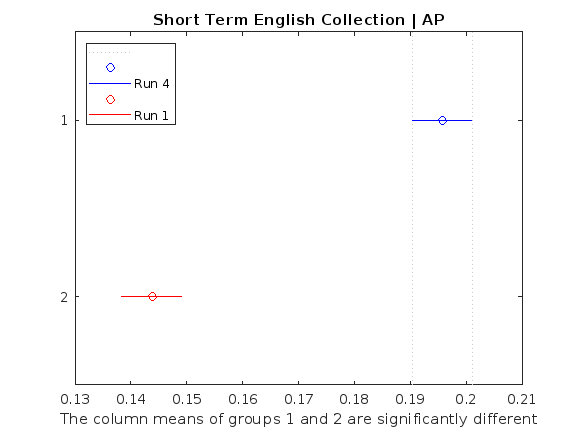
\includegraphics[width=\textwidth]{figure/StatisticalAnalysis/ANOVA 2/ap-st-en.jpeg}
        %\caption{Two-way ANOVA for Runs 2 and 4 on the Short Term English Collection}
        \label{fig:st_anova_eng_ap}
    \end{subfigure}
    \caption{Two-way ANOVA for runs 1 and 4 on the Short Term English Collection}
    \label{fig:st_anova_eng}
\end{figure}

These results are really close to the ones shown in FIgure \ref{fig:lt_anova_eng}, therefore we can consider this as confirming everything we have found until now, indicating the superiority of run 4 on both short-term and long-term Collection.

To provide additional statistical information, Tables \ref{table:st_anova_eng} and \ref{table:st_anova_eng_ap} present the results of the multiple comparisons between run 1 and run 4.

\begin{table}[!h]
    \centering
    \caption{Multiple comparisons for the Short Term English Collection}
    \label{table:st_anova_eng}
    \begin{tabular}{cccccc}
    \hline
    Run A & Run B & Lower Limit & A-B Difference & Upper Limit & P-value \\
    \hline
    4 & 1 & 0.0458 & 0.0564 & 0.0671 & 0.00 \\
    \hline
    \end{tabular}
\end{table}

\begin{table}[!h]
    \centering
    \caption{Multiple comparisons for the Short Term English Collection}
    \label{table:st_anova_eng_ap}
    \begin{tabular}{cccccc}
    \hline
    Run A & Run B & Lower Limit & A-B Difference & Upper Limit & P-value \\
    \hline
    4 & 1 & 0.0412 & 0.052 & 0.0628 & $1.05 \times 10^{-21}$ \\
    \hline
    \end{tabular}
\end{table}

Table \ref{table:st_anova_eng} shows that there is a significant difference in the \ac{nDCG} scores between run 1 and run 4 on the Short Term English Collection. 
The A-B difference, which represents the difference in \ac{nDCG} scores between the two runs, is 0.0564, indicating that run 4 performs substantially better than run 1. 
The p-value of zero further supports the significance of this difference.

These findings consistently demonstrate the superiority of run 4 over run 1 in terms of \ac{nDCG} and \ac{AP} scores in both short and long-term evaluations of the English collection.


\newpage
\enlargethispage{4\baselineskip}
\subsection{Final Considerations on Statistical Analysis}

In this section, we conducted a comprehensive statistical analysis of the retrieval performance of our system on both the French and English collections. 
We focused on evaluating the overall \ac{nDCG} and \ac{MAP} scores, as well as conducting two-way \ac{ANOVA} tests to examine the effects of different factors on the performance.

For the French collection, the analysis revealed that run 5 consistently exhibited slightly better or comparable performance compared to run 3 across all evaluation points. 
This suggests that the modifications in the stoplist made in run 5 resulted in improved retrieval effectiveness.
Still, we noticed this change introduced some instability in the temporal persistence of the system, so we cannot be sure a further expansion of the stoplist can be a promising option for future development. 

On the other hand, run 2 displayed significantly worse performance compared to the other runs. 
Recalling that run 3 and run 5 are basically improved versions of run 1 which implements query expansion and query re-ranking, we can see this as a good result: the implemented changes had a significant positive impact in our \ac{IR} system.  

Turning to the English collection, we focused on comparing runs 1 and 4. 
The results consistently demonstrated that run 4 outperformed run 1 in every aspect of the analysis. 
It achieved higher \ac{nDCG} and lower \ac{RnD} scores, indicating its superior effectiveness in retrieving relevant documents, remaining persistent at changes over time. 
Additionally, run 4 displayed a higher median \ac{MAP} score, confirming its superior overall performance in both short and long windows of time. 
These findings establish run 4 as the more successful option for retrieval on the English collection.
This is an expectable result, since it confirms what we have seen with the French collection: the implementation of query expansion and query re-ranking improved by a lot the performances of our, at the time greedy and basic, \ac{IR} system. 

The two-way \ac{ANOVA} tests further supported our conclusions. 
In the French collection, the two-way \ac{ANOVA} analysis confirmed the superiority of run 5 over run 3 in terms of \ac{nDCG} scores. 
This finding aligns with the overall comparison results. 

In the English collection, the two-way \ac{ANOVA} did not provide any new unexpected result, as the performance differences between run 1 and run 4 were consistently evident in all previous aspects of the analysis.

In summary, for the French collection run 5 exhibited slightly better or comparable performance compared to run 3, while run 2 displayed significantly worse performance. 
On the other hand, for the English collection run 4 consistently outperformed run 1 in every aspect of the analysis.

































